%===================================== CHAP 1 =================================

\chapter{Introduction}

\section{Motivation}

Studying abroad can be an important way to improve intercultural communication skills that are increasingly more important in international businesses and for cooperation between different cultures.\cite{williams2005exploring} Many students choose to go abroad by doing an exchange program or a study-abroad program. These programs usually lasts for 6-12 months where the student is studying at a university in a different country. To apply for exchange or study abroad at the Norwegian University of Science and Technology (NTNU) the students have to find and pre-approve courses which are desired to take at the university abroad. The process of planning and choosing courses is a time consuming and tedious task, where both the supervisor and student has to undergo a large amount of manual work. 

The purpose of this research, is to propose the hypothesis that significally simplyfying this process, as well as making all required information easily available would increase the interest among students to study abroad. This process can be replaced by an information system (IS) that automates a large part of the manual work, as well as intelligently suggesting proper subjects and universities to choose by using an intelligent recommendation system with the artifical intelligence (AI) methodology Cased-based Reasoning (CBR).


\section{Background}

A study by Mazzarol and Soutar\cite{mazzarol2002push} shows that students' general motivation is influenced by the amount of information on the university and its courses. Among the several factors which was reviewed in the study, the \enquote{knowledge and awareness} factor proves to be the most influencing one for choosing an international study location. Therefore, when investigation how an IS can improve this process, proper information is key. 

Several approaches has been made to replace the manual process of choosing courses with an IS. One example is by using a decision support system that advises the students on their course selection based on their program requirements and the course's prerequisites, as done at the University of Dhaka\cite{roushan2014university}. Student course recommendation can be done intelligently by using recommendation engines and data mining techniques to give relevant results. Sherpa\cite{bramucci2012sherpa} is a system that has been made especially for the goal of giving course recommendations. Data mining techniques can also be used to predict whether a student will fail or pass on a course\cite{vialardi2009recommendation}.

Software engineering varies from other fields of study by having a more practical approach to the research. This paper primarily focus on research for how the promoted IS can be implemented,  what it can do to provide a optimal contribution to NTNU, and whether it can increase the motivation for students to do a study exchange program. The following list summarize the concise research questions which this research will try to answer:

\begin{itemize}
    \item \textbf{RQ1:} How can intelligent recommendation increase students' motivation for studying abroad?
    \item \textbf{RQ1.1:} What information and features are important for an IS to be used? 
    \item \textbf{RQ2:} Is the domain of choosing subjects and universities suitable for case-based reasoning?
    
\end{itemize}

\section{Contributions}

This research's contribution will yield a new computer based artefact; specifically an IS with the goal of both motivating and making it easier for students at NTNU to apply for a study exchange program.

As implied by some of the similar systems and solutions already mentioned, this research will invent a new innovating system that could be extended to other universities. Aside from simplifying this process, the research will contribute by giving new insight and knowledge about what an IS can do to increase the motivation for students to apply for a study exchange program, and if it is possible to completely automate this process, as well as providing automated intelligent educated guesses for the most suitable and relevant courses a student should choose. Considering this research objective is primarily designed as a contribution to NTNU, who currently does most of this process manually, if this research and product proves to be successful, it will be a great contribution for NTNU. All though there exists similar systems in other universities which focus on some of the same objectives as this research, commercial-off-the-shelf (COTS) products can not be implemented, when the dependencies and infrastructure is so different for different universities.

\section{Methodology}

This study will first focus on gathering qualitative data, gained by interviewing key persons, and studying existing documents and diagrams, as well as investigating if contribution will increase motivation, which can be viewed upon as subjective and individual. Furthermore, as stated by our motivation for performing this research project, it’s hard to avoid being biased in some form. These factors all relate most closely to the interpretivism paradigm. We therefore conclude that our way of thinking throughout the research will be categorized towards this paradigm.

The major results that will be collected are the numbers for students going on exchange. As mentioned the project aims to improve the motivation for students to go on exchange and ultimately see an increase. We will collect this data by requesting statistics from NTNU on the amount of students on exchange. We will then compare this to previous measured data and the total number of students studying at that time. This data will be visualized through a graph for each measured data. Below is an example on the variables the data might be formed in. These tables will then be made into a graph showing the development. If the project has any large influence on the number of exchange students it will show in the graph.

Statistical analysis can also be done on the data of students going on exchange. It will give a clearer view of how drastic the change in exchange students were and if implementing the system really gives an significant effect. One statistical method could be used is one-way analysis of variance to test the hypothesis. 

The surveys will be conducted through online service providers that provide the framework for the survey. The answer to the survey will then be stored in an datasheet to be analysed at a later point. Some survey sites also includes simple data analysis that give more information on the data collected in a survey.

Measuring the quality of the project as a whole will be done by analysing several factors of the research and development. We will in the project analyse the qualitative data resulting from interviews and surveys on both the manifest level and latent level of analysis. This will give a better understanding on both the clear results and what we can infer or imply from the questions. 

We can use the qualitative content analysis methods presented by S. Elo and H. Kyngäs[1] for systematic, rule-guided qualitative text analysis in the interview and survey questions. This model will help preserve the advantages of quantitative analysis in the qualitative based research results. The steps for the content analysis is described in model 1[3]. 

The research in information systems varies to other fields by having a more practical approach to the research. The results are often given using empirical methods on users by doing usability testing and surveys. Knowing how to do perform the analysis in a correct way is important both for the quality of the results and the research validity. A book on empirical research methods have identified the common pitfalls and describes how to avoid them [2]. 

There is several relevant books and literature on analysis that should be read before starting evaluating the project. One of these include “Qualitative evaluation and research methods” by M. Q. Patton [4]. This book introduces method for analysis and evaluation that might prove useful in the project. 

\begin{figure}
    \centering
    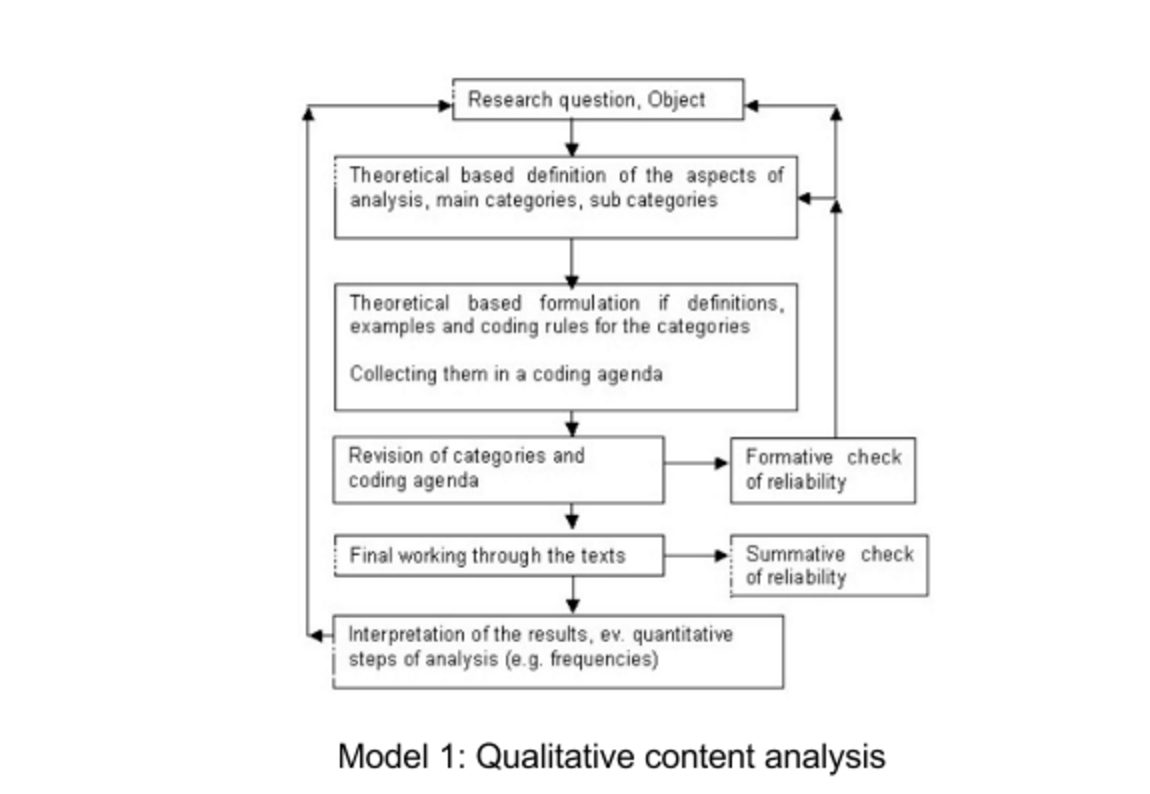
\includegraphics[width=\textwidth]{fig/method.png}
    \label{fig:my_label}
    \caption{The outlined research process\cite{oates2005researching}}
\end{figure}


\section{Chapter Descriptions}
This section will describe the different chapters of this thesis. The main focus and content will be detailed to gain a brief overview of the thesis structure. 

\subsection{Background}
This chapter presents related theory and work that has a large focus continuing in the thesis. The main focus will be on CBR and recommender systems and some of the previous implementations.  

\subsection{CBR Model}
Description of our CBR implementation. Including similarity measures, case base information and the different CBR process stages that was used. 

\subsection{System \& Architecture}
This chapter will go into detail on how the system Utsida is built. Including reasoning for the design choices. 

\subsection{Experiment \& Results}
Describes the experimental methods used to retrieve information. The information retrieved will be presented to give the background for further analysis. 

\subsection{Analysis}
This chapter will analyse and discuss the results from the previous chapter.

\subsection{Conclusion}




\cleardoublepage